% easychair.tex,v 3.1 2011/12/30
%
% Select appropriate paper format in your document class as
% instructed by your conference organizers. Only withtimes
% and notimes can be used in proceedings created by EasyChair
%
% The available formats are 'letterpaper' and 'a4paper' with
% the former being the default if omitted as in the example
% below.
%
\documentclass[procedia]{easychair}
%\documentclass[debug]{easychair}
%\documentclass[verbose]{easychair}
%\documentclass[notimes]{easychair}
%\documentclass[withtimes]{easychair}
%\documentclass[a4paper]{easychair}
%\documentclass[letterpaper]{easychair}

% This provides the \BibTeX macro
\usepackage{doc}
\usepackage{makeidx}
\usepackage{caption}
\usepackage{subcaption}
\usepackage{pgfplots}
\usetikzlibrary{patterns}
\usepackage{tikz}
\usepackage{subcaption}
\usepackage{amsmath}
\usepackage{amsfonts}
\usepackage{amssymb}
\usepackage{amsbsy}
\usepackage{amsthm}



% In order to save space or manage large tables or figures in a
% landcape-like text, you can use the rotating and pdflscape
% packages. Uncomment the desired from the below.
%
% \usepackage{rotating}
% \usepackage{pdflscape}

% If you plan on including some algorithm specification, we recommend
% the below package. Read more details on the custom options of the
% package documentation.
%
% \usepackage{algorithm2e}

% Some of our commands for this guide.
%
\newcommand{\easychair}{\textsf{easychair}}
\newcommand{\miktex}{MiK{\TeX}}
\newcommand{\texniccenter}{{\TeX}nicCenter}
\newcommand{\makefile}{\texttt{Makefile}}
\newcommand{\latexeditor}{LEd}

\def\procediaConference{99th Conference on Topics of
  Superb Significance (COOL 2014)}

%\makeindex

%% Front Matter
%%
% Regular title as in the article class.
%
\title{Traffic State Estimation Using Floating Car Data}

% \titlerunning{} has to be set to either the main title or its shorter
% version for the running heads. When processed by
% EasyChair, this command is mandatory: a document without \titlerunning
% will be rejected by EasyChair

\titlerunning{Traffic State Estimation Using  Floating Car Data}

% Authors are joined by \and. Their affiliations are given by \inst, which indexes into the list
% defined using \institute
%
\author{
    Abhinav Sunderrajan\inst{1}
\and
    Vaisagh Viswanathan\inst{1}
    \and
        Wentong Cai\inst{2}
\and
    Alois Knoll\inst{3}\\
}

% Institutes for affiliations are also joined by \and,
\institute{
  TUM CREATE,
  Singapore\\
  \email{abhinav.sunderrajan@tum-create.edu.sg, vaisagh.viswanathan@tum-create.edu.sg}
\and
   Nanyang Technological University,
   Singapore\\
   \email{aswtcai@ntu.edu.sg}\\
\and
   Technische Universit\"at M\"unchen,
   Germany\\
   \email{knoll@in.tum.de}\\
 }


\authorrunning{Sunderrajan, Viswanathan, Cai and Knoll}

\begin{document}

\maketitle

\keywords{Traffic state estimation, Simulation and modelling of transportation systems, Agent-based simulations}

\begin{abstract}
There is an increasing availability of floating car data both historic, in the form of trajectory datasets and real-time, in the form of continuous data streams. This paves the way for several advanced traffic management services such as current traffic state estimation, congestion and incident detection and prediction of the short-term evolution of traffic flow. In this paper, we present an analysis of using probe vehicles for reconstructing {\it traffic state}. We employ detailed agent-based microscopic simulations of a real world expressway to estimate the state from {\it floating car data}. The probe penetration required for accurate traffic state estimation is also determined.
\end{abstract}



\section{Introduction}
\label{sect:introduction}

 Floating cars refer to moving probe vehicles which act as traffic sensors by providing information regarding their position $\alpha$ (in terms of coordinates) and speed $v_{\alpha}$ at regular intervals. The locations provided via GPS receivers can be map-matched to roads on a map. In turn this map-matched data can be used to reconstruct traffic state constituting the macroscopic quantities density $\rho$, flow $Q$ and local speed $\bar{V}$. Identifying regions of uniform flow and density will help determine traffic patterns of interest such as jams, stop-and-go waves and changes in traffic flow especially in the face of events such as accidents. In this paper we develop a methodology for aggregating floating car data (FCD) for accurate traffic state reconstruction. The minimum probe penetration required for determining the traffic state is also determined by simulating different traffic flow regimes on a real world expressway.
 
 Reconstruction of traffic state in real-time using FCD (in the form of data streams) will also enable initializing data driven traffic simulations for short term predictions of flow. This can lead to a {\it symbiotic traffic simulation platform}~\cite{aydt2012symbiotic} where the simulation system benefits from the real time data provided by the physical system (the road network) which in turn benefits through mechanisms such as dynamic ramp metering and congestion aware routing~\cite{yang2000simulation}. 
 
Reconstructing traffic state from probe vehicles has been previously discussed in papers such as ~\cite{kerner2005traffic,hong2007spatial} and~\cite{de2008traffic}. In this work we attempt to determine traffic density and flow  traditionally computed through stationary devices such as loop detectors~\cite{cheung2005traffic} and video cameras~\cite{coifman1998real}, using FCD. Towards this end the contributions of this paper are -

\begin{enumerate}
\item  A methodology for obtaining aggregated macroscopic (speed, density and flow) quantities from the microscopic FCD consisting of $(\alpha, v_{\alpha})$.
\item  An estimation of the minimum percentage of probe vehicles required for the macroscopic traffic state reconstruction  under different traffic flow regimes. 
\end{enumerate}

 
 \section{Existing Work}
 \label{sec:lit-review}
 
 Using FCD as a means for estimating travel times and traffic state has received much attention over the years. Papers such as~\cite{de2008traffic} and~\cite{nanthawichit2003application} compute the average travel time on roads from the average speed of the probes on that road. Techniques such as artificial neural networks are used for short term predictions by using weighted aggregates of the past patterns~\cite{de2008traffic}. While using the trajectories of probe vehicles to detect events such as congestion and accidents has been discussed in~\cite{asakura2015incident}.  
 
 The percentage of probe vehicles required for reliable travel-time estimation has been discussed in papers such as~\cite{dai2003simulation} and ~\cite{hong2007spatial}. The work in~\cite{kerner2005traffic} is concerned with estimating the percentage of probe vehicles for accurately determining the travel-time across the road-network links. Based on numerical simulations (details of the simulation model are not provided), the authors conclude that $1.5\%$ penetration of probe vehicles are needed for accurate travel time estimation. 
 
 While the authors of~\cite{hong2007spatial} estimate the  probe penetration (to be around $2\%$) and the sampling period to maximize traffic information by determining {\it traffic time and space correlations}. Two spots are correlated in space if the correlation of average speeds in both the spots exceeds a threshold. Thus, the traffic condition in a spot without measurements can be estimated if the condition in a correlated spot is known, thus influencing probe penetration. Likewise the correlation time measures the period over which the traffic conditions remain correlated in a spot hence influencing the sampling period. The traffic time and space correlations were measured using microscopic simulations. The details of the simulation parameters are not provided.
 
 Similarly~\cite{dai2003simulation} defines confidence intervals for accuracy in terms of average speed and travel times across the links apart from spatial coverage as a function of probe penetration. The authors conclude that $3\%$ to $5\%$ probe penetration is sufficient for confidence levels of $90\%$ and above. 
 
 To the best of our knowledge, there have been no attempts made at estimating traffic flow and density from FCD. This is generally due to the papers focusing mainly upon estimating travels times from FCD which is in contrast to the requirements of a symbiotic traffic simulation platform requiring knowledge of the current state in terms of $\rho, Q$ and $\bar{V}$. Further, most employ macroscopic models which do not take into account the heterogeneous driving characteristics and vehicle lengths and instabilities arising due to lane changes. This results in optimistic conclusions on the minimum probe penetration required. In this work we show that, provided sufficient probe penetration, the traffic state constituting average speed and more importantly density (and flow) can be reliably measured. 
 
 
 \section{Methodology}
 \label{sec:Methodology}
 
 For determining the methodology for spatial aggregation of FCD and the minimum probe penetration for accurate traffic state estimation, we employ agent-based microscopic traffic simulations. Microscopic simulations  of real world expressway were employed owing to lack of real-world floating car data.
 
 Once the $(\alpha, v_{\alpha})$ pairs for the road stretch simulated is obtained, an algorithm for partitioning the FCD is required for determining the aggregated values of traffic density and in turn, the flow. In order to do this, the partitioned regions must be microscopically large enough to contain sufficient samples of $(\alpha, v_{\alpha})$ pairs and be macroscopically small to determine traffic patterns of interest such as congestion and variations in flow~\cite{Traffic_Flow_Treiber}. 
 
 The first method for spatial aggregation evaluated, naively divides the expressway into uniform chunks of size $1.0$ km each resulting in $13$ segments in total. The second method evaluated makes use of the topology of the expressway and divides it into segments between on/off ramp pairs. The final approach divides the expressway into $M$ segments such that the variance of the speeds within all segments are minimized. Formally, the goal is to find sections $S_{1}$, ... , $S_{J}$ that minimize the total variance of the speeds given by
 $\sum\limits_{j=1}^{J} \sum\limits_{\substack{i \in S_{j}}} (v_{i}-\bar{V}_{S_{J}})$. Where $\bar{V}_{S_{J}}$ represents the average speed in section $S_{j}$. This computationally hard optimization problem (due to the infinite number of ways in which the expressway can be divided into $J$ sections) is solved using a top down greedy approach known as {\it recursive binary splitting}~\cite{james2013introduction}. The constructed binary tree is split until a minimum of $10$ samples are present in each leaf node. The tree so grown is pruned (to prevent over-fitting) using {\it cost-complexity pruning}~\cite{james2013introduction}.
 
 The efficacy for spatial aggregation is determined based on the best model fit that can be obtained for $\rho$ as a function of $\bar{V}$. To quantify the reliability of the model, we make use of the {\it $R^2$ Statistic}. This metric used henceforth in this paper is a measure of model fit in the form of a proportion of variance explained by the model~\cite{james2013introduction}. It takes a value between $0.0$ and $1.0$ and a value close to $1.0$ indicates that a large proportion of the variability in the density is explained by the predictor, which in this case is the speed $\bar{V}$.
 
 Once the relationship between $\rho$ and $\bar{V}$ is established, we look at quantifying the accuracy of traffic state estimation as a function of probe vehicle penetration for different traffic conditions. This helps to determine the minimum probe penetration required.
 
\section{Experiments}
\label{sec:design_expt}

Microscopic models describe traffic from the perspective of individual {\it driver-vehicle units} (DVUs). These high-fidelity simulations should ideally capture heterogeneities in traffic in terms of different vehicle classes (e.g. cars, trucks) and driver behaviors (e.g. intelligent, aggressive). Further, the microscopic simulations employed for this study also model stochastic lane changes thus helping to reconstruct the spatiotemporal state of traffic with far greater accuracy in comparison to macroscopic models. The movement of driver-vehicle units are characterized by acceleration models for longitudinal motion and lane change models for lateral movement along the road. In this section, we provide the details of our microscopic simulation and of the real world expressway in Singapore we simulate.


\subsection{Traffic Simulation}
\label{sec:probabilistic}

The traffic simulation we have employed, is based on the {\it SEMSim} platform~\cite{zehe2015semsim}. SEMSim is a high fidelity agent-based microscopic simulation. It uses the {\it Intelligent Driver Model}~(IDM)~\cite{treiber2010open} and MOBIL~\cite{kesting2015general} as the acceleration and lane change models respectively. 

The IDM is an accident free model which ensures that a vehicle attains the desired velocity at free flow and maintains the safe bumper to bumper distance to the leading vehicle. It also ensures that the acceleration is an increasing function of the speed and distance to the leading vehicle and a decreasing function of its speed. MOBIL, the lane change model ensures that the resultant accelerations and decelerations for a vehicle and its followers in the old and new lanes does not exceed a safe threshold. A lane change is done only if a vehicle gains speed without violating the safety and inconvenience (to the old and new followers) criteria.


The simulation takes as input a road network detailing the lanes constituting the roads to be simulated. Road segments that don't have a preceding road segment are considered {\it sources} and those without a subsequent segment are {\it sinks}. The traffic thus flows from the sources to the sinks. Vehicles are created at each source as a Poisson process based on the equation $nextTime_{s}= \frac{-ln U}{\lambda_{s}}$. The parameter $nextTime_{s}$ represents the time of arrival of a vehicle on a source road $s$.  The mean inter-arrival time for $s$ (in seconds) is given by $\lambda_{s}$. The parameter $U$ is a random number between $0$ and $1$. The mean inter-arrival times $\lambda_{s}$ of vehicles on a source link $s$ controls the average vehicle density on all roads simulated. It represents the expected value of the number of agents entering the simulation via a source road. The route taken by each DVU is determined  based on static turn ratios specified at each intersection. Other inputs to the simulation include time, number of agents and probability distribution of other model parameters.


\subsection{The Simulated Environment}
\begin{center}
\begin{figure}[!htbp]
    \centering
    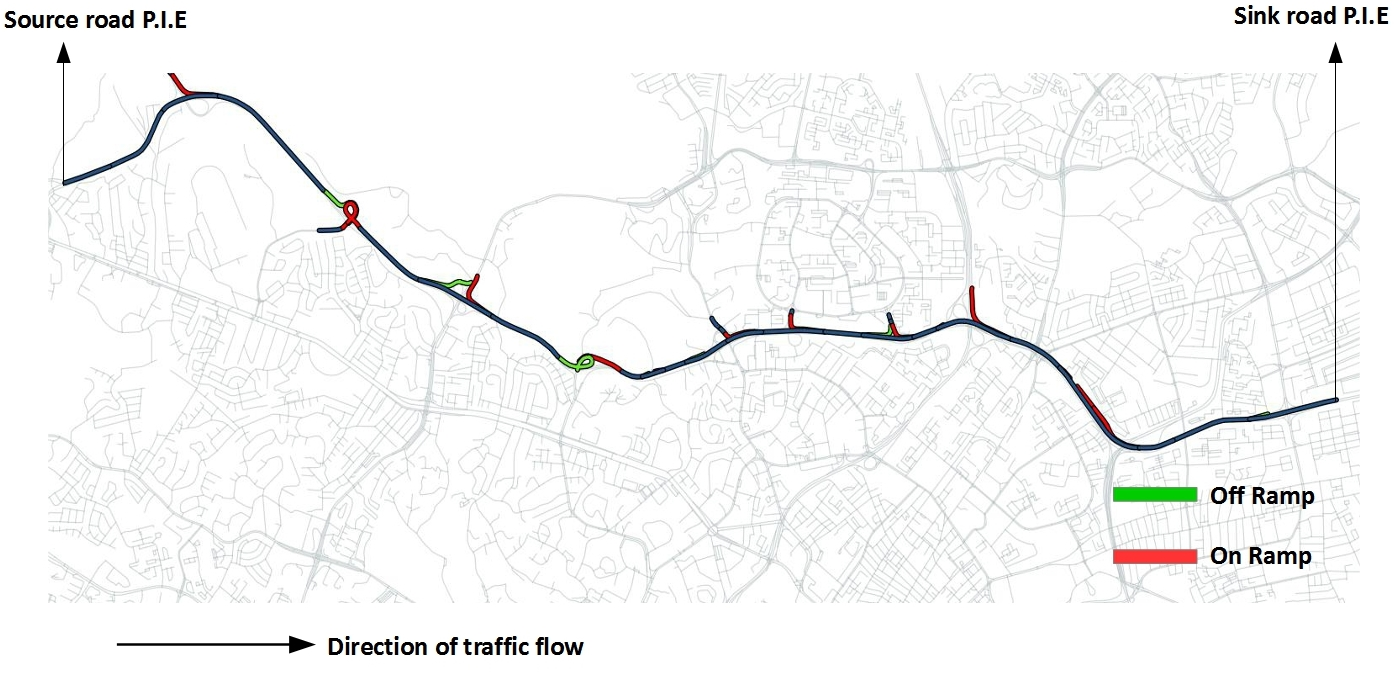
\includegraphics[scale=0.40]{graphs/PIE.jpg}

    \caption{Simulated section of P.I.E (Singapore) and location of all on/off ramps.}
    \label{fig:pie-changi}
  \end{figure}
\end{center}
For the experiments in this paper, we simulated a $13$ km stretch of P.I.E (Pan Island Expressway) in central Singapore (Figure~\ref{fig:pie-changi}) with all on and off ramps. The on ramps and the first P.I.E link are sources, while all off ramps and the last link on P.I.E are sinks. Refer to the Table~\ref{fig:pie-changi} for the location of all on/off ramps (or {\it static bottlenecks}) starting from the beginning of the first road-segment on P.I.E. The average distance between two bottlenecks is around $565$ m along this stretch of P.I.E. The turn ratios for all off-ramps is kept constant at $0.25$. This implies that $25\%$ of all vehicles exit at a given off ramp while the remaining $75\%$ of the vehicles continue to travel on the main expressway. The number of lanes in the simulated stretch of the expressway varies between $3$ and $6$.



\begin{table}[!ht]
 \centering
\begin{tabular}[b]{ccc}\hline
      {\bf DISTANCE} (m) & {\bf RAMP TYPE} \\ \hline
     583.98 & On Ramp \\ 
     1973.35 & Off Ramp \\ 
     2489.87 & On Ramp \\ 
     3261.27 & Off Ramp \\ 
     4071.9 & On Ramp \\ 
     4834.84 & Off Ramp \\ 
     5531.18 & On Ramp \\ 
     5743.11 & Off Ramp \\ 
     5965.29 & On Ramp \\ 
     6207.74 & Off Ramp \\ \hline
     \end{tabular}
     \quad
     \begin{tabular}[b]{ccc}\hline
       {\bf DISTANCE} (m) & {\bf RAMP TYPE} \\ \hline
     7025.15 & On Ramp \\ 
     7658.4 & On Ramp \\ 
     8040.83 & Off Ramp \\ 
     8554.28 & On Ramp \\ 
     8807.94 & Off Ramp\\ 
     9591.84 & On Ramp \\ 
     10148.24 & Off Ramp \\ 
     11286.2 & On Ramp \\ 
     11637.04 & On Ramp \\ 
     12438.23 & Off Ramp \\  \hline
    \end{tabular}
      \caption{Location of all On/Off ramps along the expressway.}
      \label{table:on-off-ramp}
\end{table}


 

\subsection{Simulation Parameters}
\label{sec:simparam}

The microscopic traffic simulation of P.I.E  was initialized with the parameters listed in Table~\ref{table:sim-param}. Parameters such as $a$, $b$ and $l_{i}$ are modeled as distributions to take into account heterogeneous driving behaviors and vehicle classes respectively. In order to obtain a ballpark figure for congestion in terms of vehicle density, we make use of the simplest of the {\it Lighthill Whitham Richards} (LWR) models using a {\it triangular fundamental diagram}~\cite{Traffic_Flow_Treiber}. The {\it critical density} for congested traffic $\rho_{c}$, according to the LWR model is given by $\frac{I}{V_0\times T+l_{eff}}$. Here $l_{eff}$ represents the minimum distance headway which is the sum of average vehicle length and minimum gap $s_{0}$. Vehicle density exceeding $\rho_{c}$ generally implies a congested traffic flow regime. 

\begin{table}[!htbp]
\centering

\begin{tabular}{ccc}\hline
\textbf{\begin{tabular}[c]{@{}c@{}}Simulation\\ parameter\end{tabular}} & \textbf{Description}                                                                               & \textbf{Value}                                                                                \\ \hline \\
ST                                                                      & Simulation time                                                                                    & 7200 sec                                                                                      \\
$s_{0}$                                                                 & \begin{tabular}[c]{@{}c@{}}Minimum bumper-to-bumper distance \\ to the front vehicle.\end{tabular} & $2.0$ m                                                                                       \\
T                                                                       & Time gap to preceding agent                                                                        & $1.4$ sec                                                                                     \\
$l_{i}$                                                                       & Vehicle length                                                                  & \begin{tabular}[c]{@{}c@{}}Normal distribution with \\ $\mu=3.0$ m and $\sigma=0.1$ m\end{tabular} \\
$V_{0}$                                                                 & Desired speed of agent                                                                            & $20$ m/s                                                                                      \\
a                                                                       & Maximum acceleration term for IDM                                                                  & \begin{tabular}[c]{@{}c@{}}Uniform distribution between \\ $1.2$ and $1.6~m/s^2$\end{tabular} \\
b                                                                       & Maximum deceleration term for IDM                                                                 & \begin{tabular}[c]{@{}c@{}}Uniform distribution between \\ $1.8$ and $2.2~m/s^2$\end{tabular} \\
$p_{0}$                                                                 & Politeness factor for MOBIL                                                                       & 0.3                                                                                           \\
$\Delta a_{th}$                                                         & Lane change threshold for MOBIL                                                                   & $0.3 ~m/s^2$                                                                        \\ \hline          
\end{tabular}
\caption{The microscopic simulation parameters}
\label{table:sim-param}
\end{table}



Based on the parameters listed in Table~\ref{table:sim-param}, $\rho_{c}$ works out to around $31$ vehicles/km/lane. Thus we consider traffic greater than $93$ vehicles/km, (assuming the minimum of three lanes) as congested. In fact, each traffic scenario (discussed later) is also characterized based on the average vehicle density during the simulation period of $2$ hours. It is to be noted that the LWR based triangular fundamental diagram overestimates the critical density since it ignores vehicular interactions such as lane changes and assumes homogeneous traffic, but nevertheless serves as a rough estimate for congestion.
 
  \subsection{Simulation Scenarios}
  \label{sec:scenarios}
  
  
  
  The traffic density ($\rho$) in number of vehicles/km across the expressway is controlled by varying the average inter-arrival rates at all sources along P.I.E. The density of the entire expressway is computed at the end of the two hour simulation by counting the number of distinct agents per kilometer of the road.  To simulate heavy congestion along P.I.E the parameter $\lambda_{s}$  for all on-ramps was set to a uniform random number between $2.0$ sec and $2.5$ sec (representing a flow of $1800$-$1440$ vehicles/hour) while  $\lambda_{s}$ for the first and only source link of P.I.E was set to $1.0$ sec (3600 vehicles per hour).  The sampling period of all probe vehicles unless stated otherwise is $1$ second, i.e. the probe vehicles provide information regarding their speed and position every second.
 
 \begin{figure}[!htbp]
      \centering
          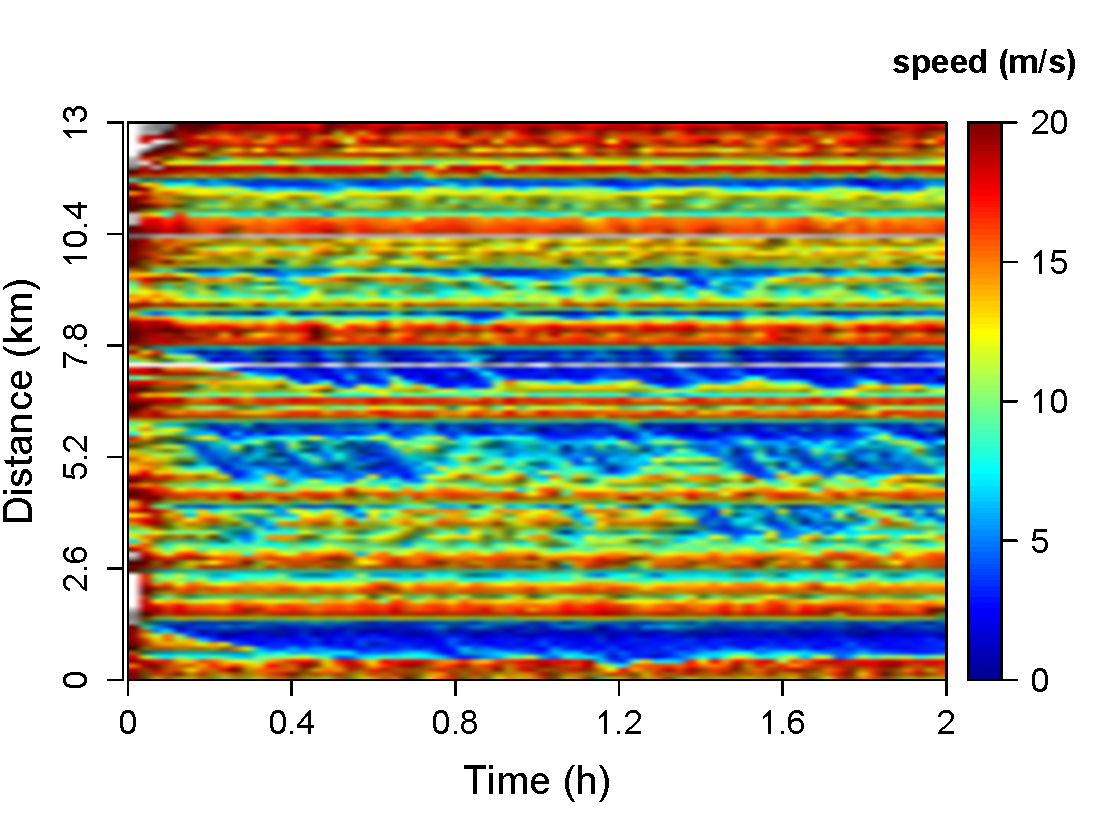
\includegraphics[clip=true,trim=0cm 0cm 0cm 1.5cm,scale=0.39]{graphs/Simulated/Heavy-Traffic}
      	\caption{Microscopic simulation of heavily congested traffic at 110 veh/km, speed in (m/s)}
      	 \label{fig:heavy-traffic}
   \end{figure}
   
   
   \begin{figure*}[!htbp]
      \begin{subfigure}[c]{.47\textwidth}
      \centering
       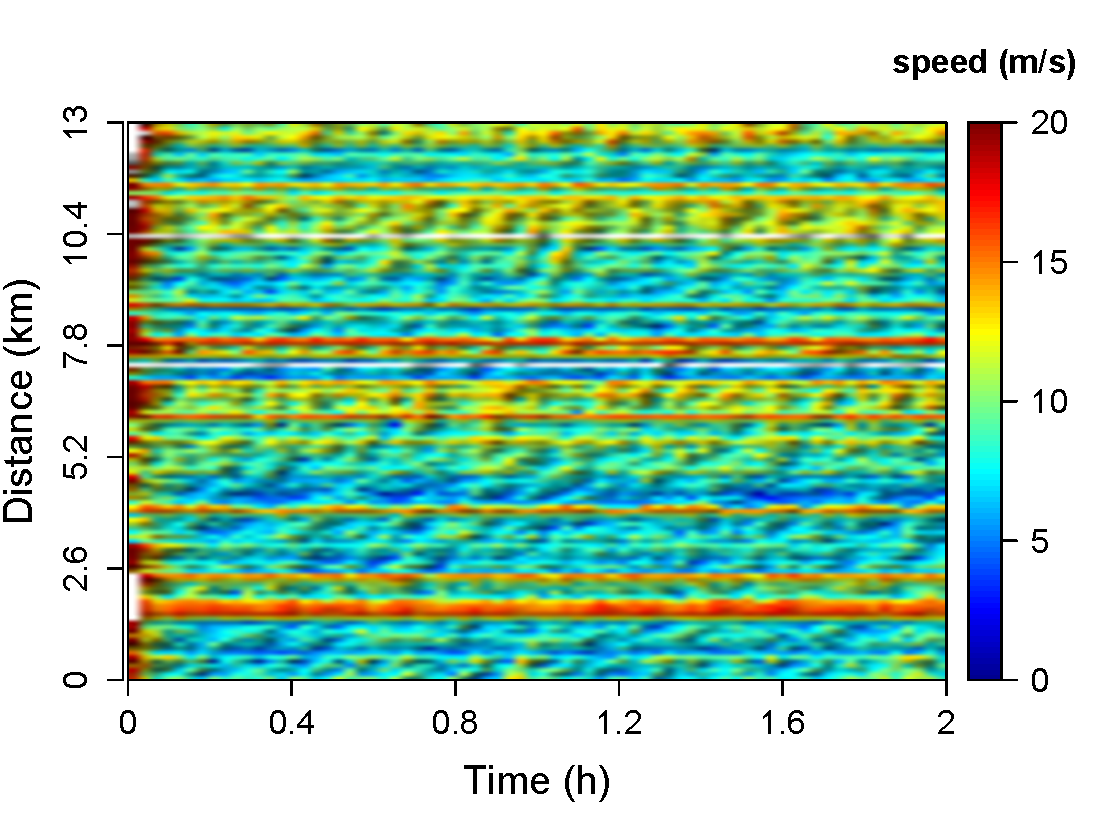
\includegraphics[clip=true,trim=0cm 0cm 0cm 1.5cm,scale=0.36]{graphs/Simulated/Partial-Congestion}
       \caption{Average density of 78 vehicles/km}
       \label{fig:partially-congested-traffic}
      \end{subfigure}
       \hspace*{\fill}
      \begin{subfigure}[c]{.47\textwidth}
       \centering
        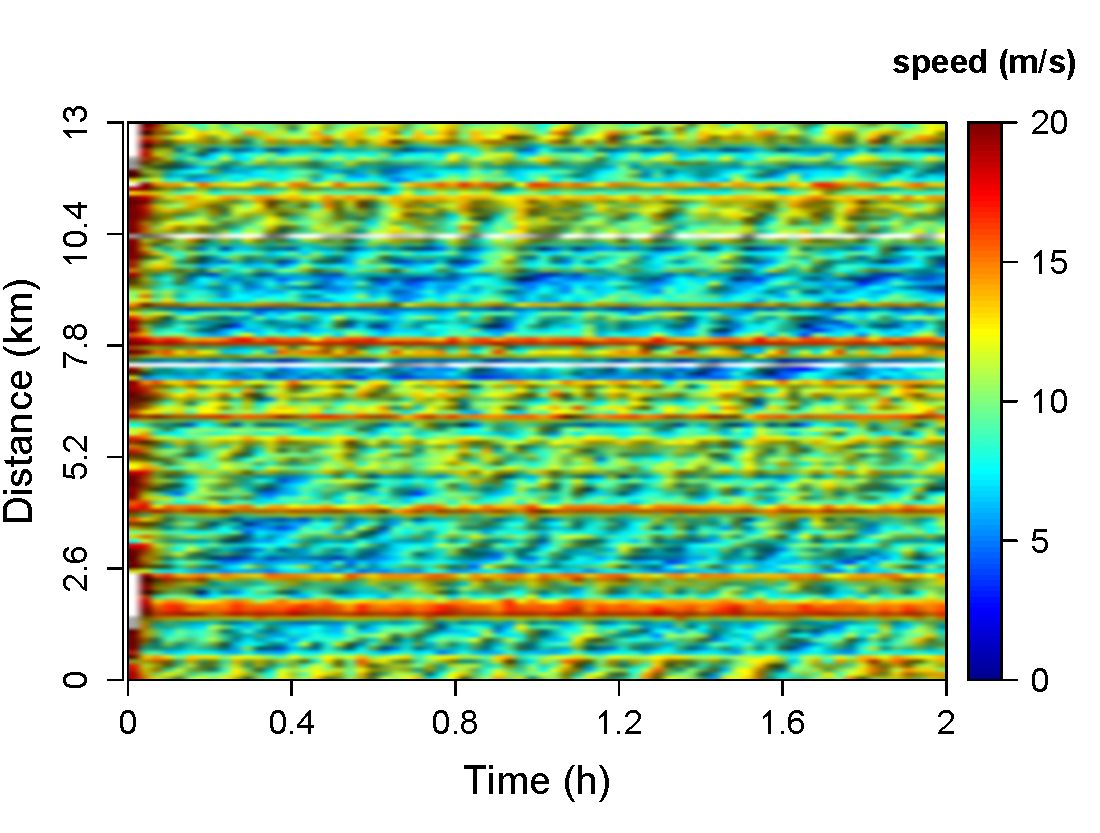
\includegraphics[clip=true,trim=0cm 0cm 0cm 1.5cm,scale=0.36]{graphs/Simulated/Medium-Traffic}
        \caption{Average density of 65 vehicles/km}
        \label{fig:medium-traffic}
       \end{subfigure} 
      \caption{Microscopic simulation of partial and minimal congestion on P.I.E, speed in (m/s)}
      \end{figure*}
     
 
 Figure~\ref{fig:heavy-traffic} shows the spatiotemporal state of P.I.E in a heavily congested state. The heat map represents the speed profiles of all the agents averaged over space and time intervals of $50$ meters and $1$ minute. Traffic build up in the form of blue bands are clearly visible in the regions where on and off ramps intersect along the main P.I.E expressway. The average traffic density along the main expressway (ignoring the on/off ramps) during the time period of simulation was around $110$ vehicles/km which is greater than the critical density $\rho_{c}$ for P.I.E.
 
 Figures~\ref{fig:partially-congested-traffic} and~\ref{fig:medium-traffic}  shows the spatiotemporal state of P.I.E during partial congestion and non-peak traffic at  average densities of $78$ and $65$ vehicles/km respectively. These scenarios as discussed in Section~\ref{subsec:penetration} will be used to determine the minimum probe penetration required for accurate traffic state estimation using FCD. Note that  three scenarios simulated in Figures~\ref{fig:heavy-traffic} through~\ref{fig:medium-traffic} assume a $100\%$ probe penetration. 
 


\section{Results}
\label{sec:experiments}

In this section, we reconstruct the macroscopic traffic state of P.I.E by aggregating the speed profiles of probe vehicles based on the three different spatial aggregation techniques discussed in Section~\ref{sec:Methodology}. We also determine the minimum probe penetration required for accurate traffic state estimation.

\subsection{Spatial Aggregation of FCD}
\label{subsec:partitioning}


 Figure~\ref{fig:splitting-100m} shows the plot of $\rho$(in vehicles/km) as function of $\bar{V}$ when the P.I.E is divided into equal sized segments of length $1.0$km. The method does not take
 into account the topography of P.I.E nor does it try to identify regions with a homogeneous distribution of speeds. While Figure~\ref{fig:splitting-pie} shows the $\rho$ vs $\bar{V}$ graph by aggregating FCD based on the $25$ road segments comprising the P.I.E stretch simulated. Both the figures clearly establish an exponential relationship (based on the linear regression fit) between $\bar{V}$ and $\rho$ despite significant bias.
 
 
\begin{figure}[!htbp]
\begin{subfigure}{.5\linewidth}
\centering
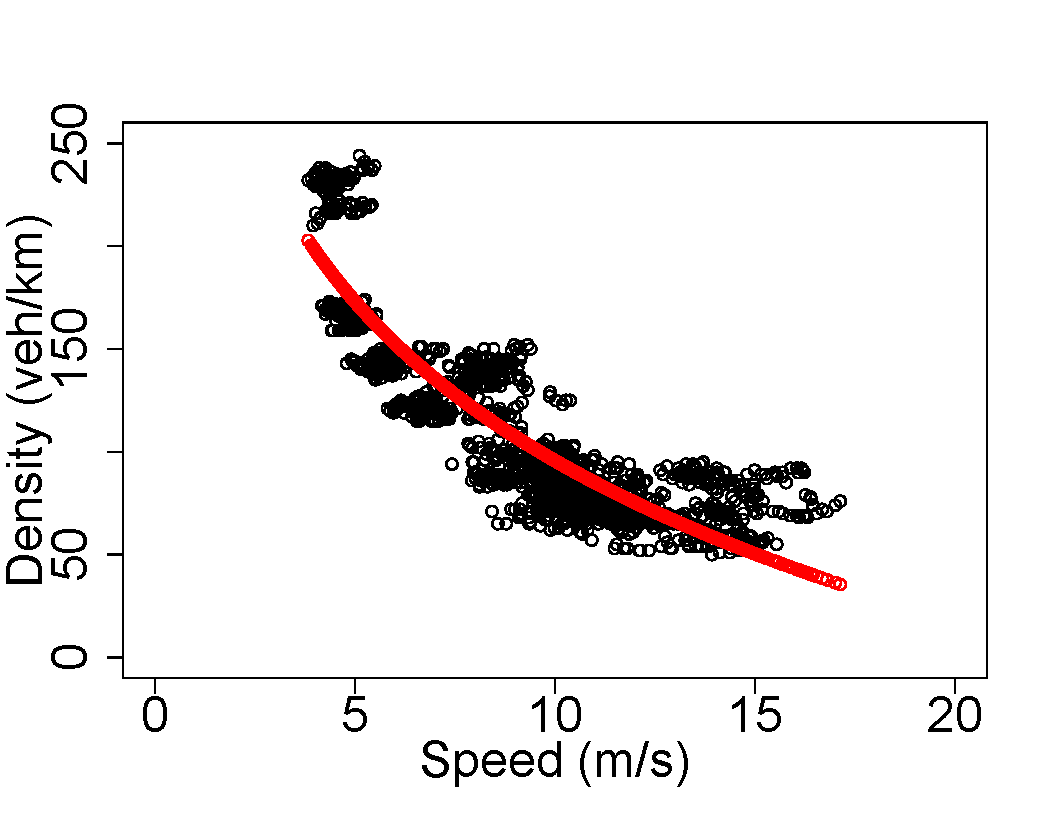
\includegraphics[clip=true,trim=0.1cm 0cm 0.0cm 1.5cm,scale=0.35]{graphs/Simulated/density-vs-speed-1000m}
\caption{13 uniform partitions of length 1.0 km}
\label{fig:splitting-100m}
\end{subfigure}%
\begin{subfigure}{.5\linewidth}
\centering
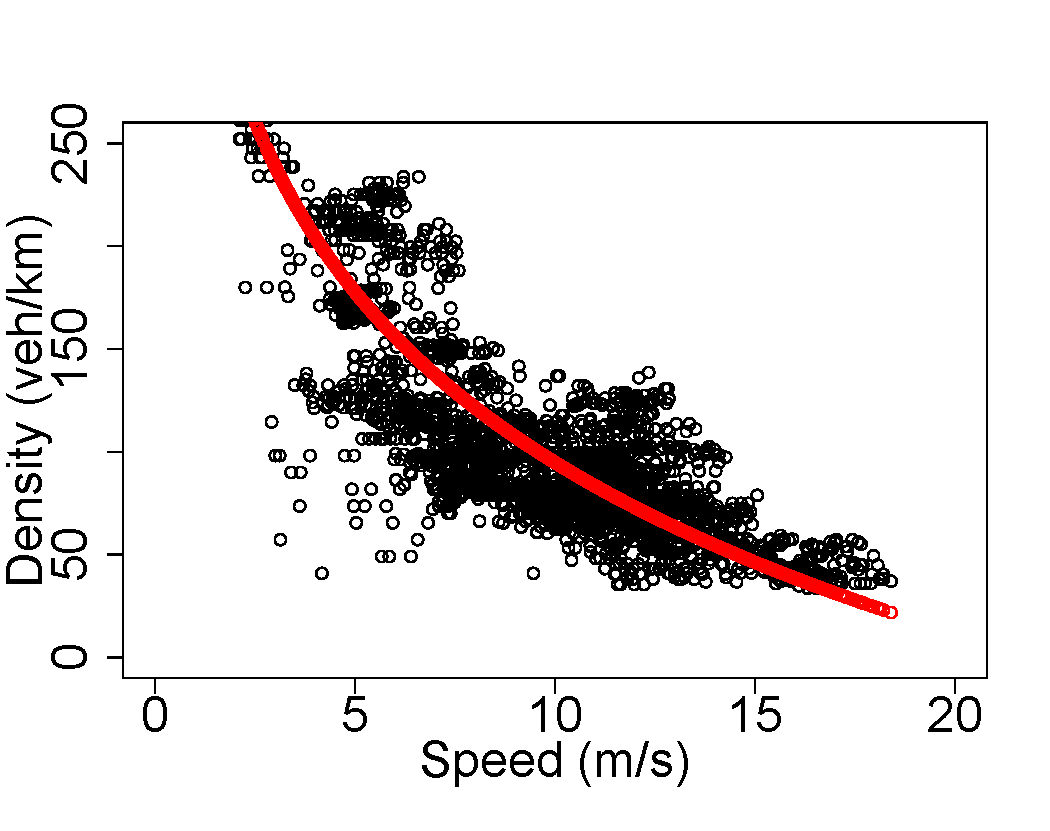
\includegraphics[clip=true,trim=0.1cm 0cm 0.0cm 1.5cm,scale=0.35]{graphs/Simulated/density-vs-speed-pie}
\caption{25 P.I.E road segments used as partitions}
\label{fig:splitting-pie}
\end{subfigure}\\[1ex]
\begin{subfigure}{\linewidth}
\centering
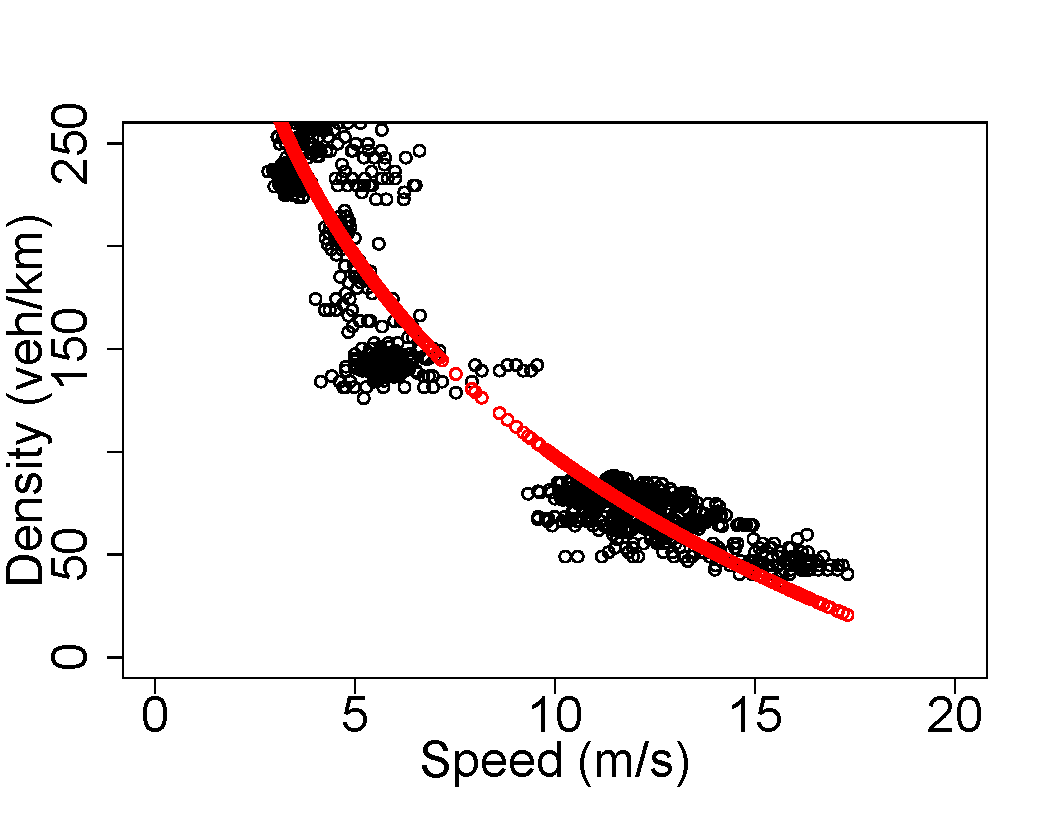
\includegraphics[clip=true,trim=0.1cm 0cm 0.0cm 1.5cm,scale=0.35]{graphs/Simulated/density-vs-speed-dt}
\caption{12 segments using recursive binary splitting}
\label{fig:splitting-dt}
\end{subfigure}
\caption{Density vs Speed for different spatial partitioning mechanisms}
\label{fig:partition-highway}
\end{figure}
 
 
 
  The recursive binary partitioning approach (Section~\ref{sec:Methodology}), divides P.I.E into  homogeneous partitions (numbering $12$ in this case) based on the speed profiles of probe vehicles. Figure~\ref{fig:splitting-dt} further establishes the exponential relationship between $\rho$ and $\bar{V}$ with much lesser noise in comparison to splitting using the two aforementioned approaches. The exponential relationship between $\rho$ and $\bar{V}$ in agreement with the {\it Underwoods's exponential model}~\cite{greenshields1961quality}. We thus fit a linear model as shown in Equation~\ref{eq:model} for estimating traffic density from average speed. The coefficients $\beta_{0}$ and $\beta_{1}$ are the least squares coefficient estimates for linear regression.

\begin{equation} 
\label{eq:model}
\rho= \beta_{0}+\beta_{1}\times log(\bar{V})
\end{equation}
 
In the next section we show that the recursive binary splitting approach is the better method for spatial aggregation of the  $(\alpha, v_{\alpha})$ pairs considering lesser levels of probe penetration.


  
\subsection{Probe Penetration for Effective Density Estimation}
\label{subsec:penetration}

In this section, we determine the accuracy of the exponential speed density model (Equation~\ref{eq:model}) at different levels of probe penetration. This helps determine the minimum probe penetration required for the three different traffic flow regimes discussed in Section~\ref{sec:scenarios}. We expect the accuracy of the exponential speed-density model (Equation~\ref{eq:model}) to decrease as the probe penetration decreases. The dip in accuracy can be attributed to significant variation in the speed of vehicles in different lanes owing to entry and exit of vehicles at on/off ramps, heterogeneous driver vehicle characteristics and stochastic lane changes. The aforementioned instabilities in traffic flow are modeled in the microscopic simulations as explained in Section~\ref{sec:design_expt}. 


\begin{figure}[!htbp]
      \centering
      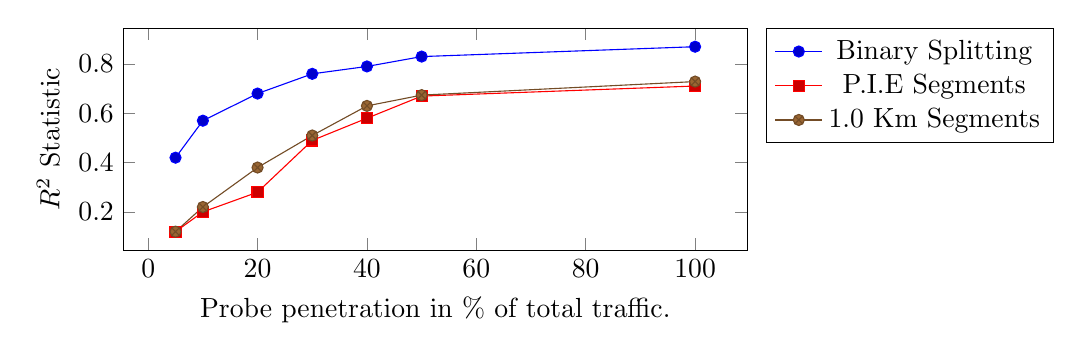
\begin{tikzpicture}
      \begin{axis}[width=9.5cm,height=4.4cm,
      	xlabel={Probe penetration in \% of total traffic.},
      	ylabel={$R^2$ Statistic},
      	legend pos=outer north east
      ]
      \addplot coordinates {
      	(100,0.87)    (50,0.83)   (40,0.79)
      	(30,0.76)  (20,0.68)  (10,0.57)  (5,0.42)	
      };
      
       \addplot coordinates {
       	(100,0.71058)    (50,0.6697562)   (40,0.58)
       	      	(30,0.49)  (20,0.28)  (10,0.2)  (5,0.12)   
       };
       
        \addplot coordinates {
              (100,0.728632)    (50,0.6736837)   (40,0.63)
                    	(30,0.51)  (20,0.38)  (10,0.22)  (5,0.12)   
         };
       
      \legend{Binary Splitting, P.I.E Segments, 1.0 Km Segments}
      \end{axis}
      \end{tikzpicture}
      \caption{$R^2$ Statistic vs probe penetration for heavily congested traffic}
      \label{fig:error-vs-penetration}
      \end{figure}



Figure~\ref{fig:error-vs-penetration} plots the $R^2$ Statistic of the exponential model (Equation~\ref{eq:model}) as a function of probe penetration for the three different aggregation methodologies discussed in the previous section. The results show the averaged $R^2$ Statistic for five different two minute sub intervals of the two hour simulation of the heavily congested traffic in~Figure~\ref{fig:heavy-traffic}. The $R^2$ statistic expectedly shows a downward trend as probe penetration decreases for all three aggregation methodologies. Figure~\ref{fig:error-vs-penetration} clearly shows binary splitting  to be a superior approach for spatial aggregation enabling a reasonable estimate of $\rho$ even at a probe penetration as low as $5\%$.  

    \begin{figure}[!htbp]
      \centering
      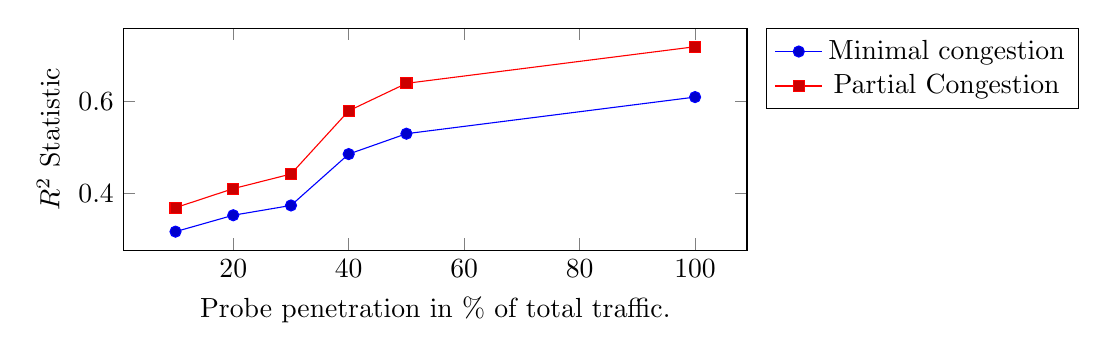
\begin{tikzpicture}
      \begin{axis}[width=9.5cm,height=4.4cm,
      	xlabel={Probe penetration in \% of total traffic.},
      	ylabel={$R^2$ Statistic},
      	legend pos=outer north east
      ]
      \addplot coordinates {
           	(100,0.61)    (50,0.53)   (40,0.4854701)
           	(30, 0.373258)  (20,0.3518749)  (10,0.3160389)	
           };
           
            \addplot coordinates {
            	(100,0.72)    (50,0.64)   (40,0.58)
            	      	(30,0.4419)  (20,0.41)  (10,0.368363)   
            };
      \legend{Minimal congestion, Partial Congestion}
      \end{axis}
      \end{tikzpicture}
      \caption{$R^2$ Statistic vs probe penetration for partial and minimal congestion}
      \label{fig:error-other-scenarios}
      \end{figure}


 Figure~\ref{fig:error-other-scenarios} plots the $R^2$ Statistic (of the exponential model fit) for recursive binary partitioning approach as a function of probe penetration for the traffic conditions shown in Figures~\ref{fig:partially-congested-traffic} and~\ref{fig:medium-traffic}. It is interesting to note that the accuracy of the model (Equation~\ref{eq:model}) decreases as the level of congestion decreases. This can be explained by the fact that vehicles generally travel at uniform speeds during heavy congestion (refer Figure~\ref{fig:heavy-traffic}) and during free flow resulting in minimum variance of speeds across lanes. While partially congested traffic regimes in Figures~\ref{fig:partially-congested-traffic} and~\ref{fig:medium-traffic} generally tend to have a far greater variance in speed due to vehicles traveling at varying speeds in different lanes.
 

\subsection{Flow estimation and temporal aggregation of FCD}

  \begin{figure*}[!htbp]
   \begin{subfigure}{.45\textwidth}
  \centering
           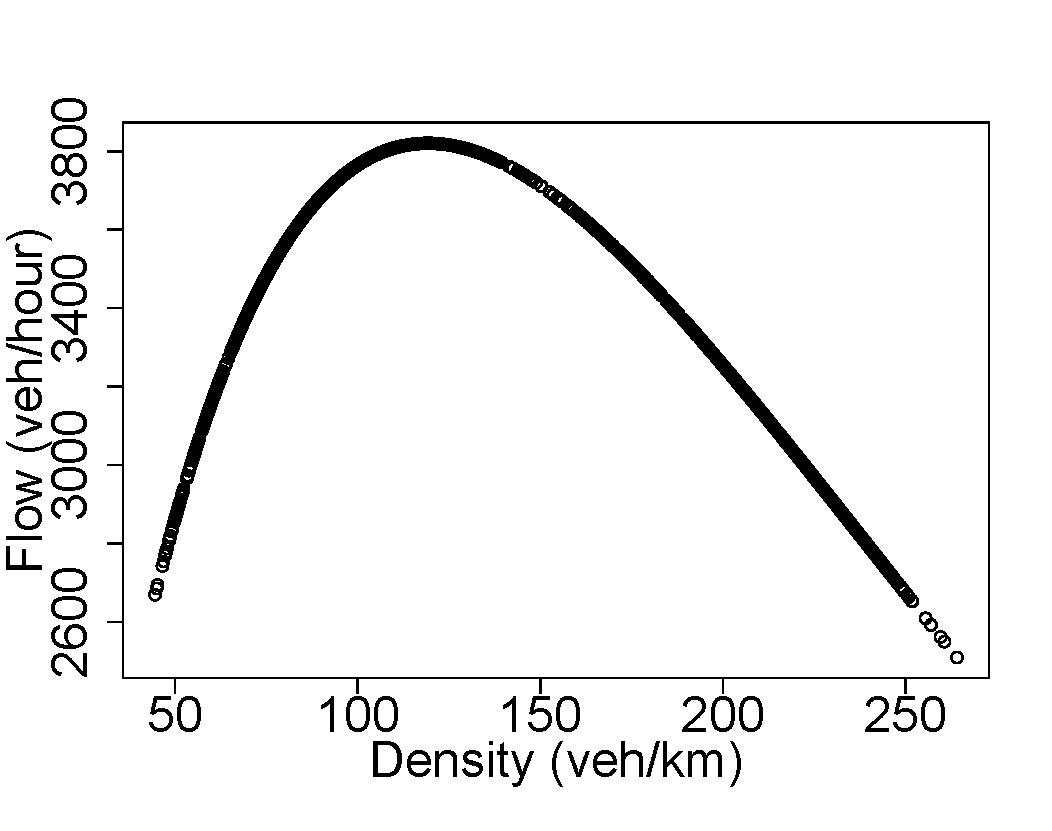
\includegraphics[clip=true,trim=0cm 0cm 0cm 2.0cm,scale=0.27]{graphs/Simulated/flow-vs-density}
       	\caption{Fundamental diagram of IDM using the density speed estimates.}
       	 \label{fig:flow-density}
   \end{subfigure}
    %\hspace*{\fill}
   \begin{subfigure}{.5\textwidth}
     \centering
             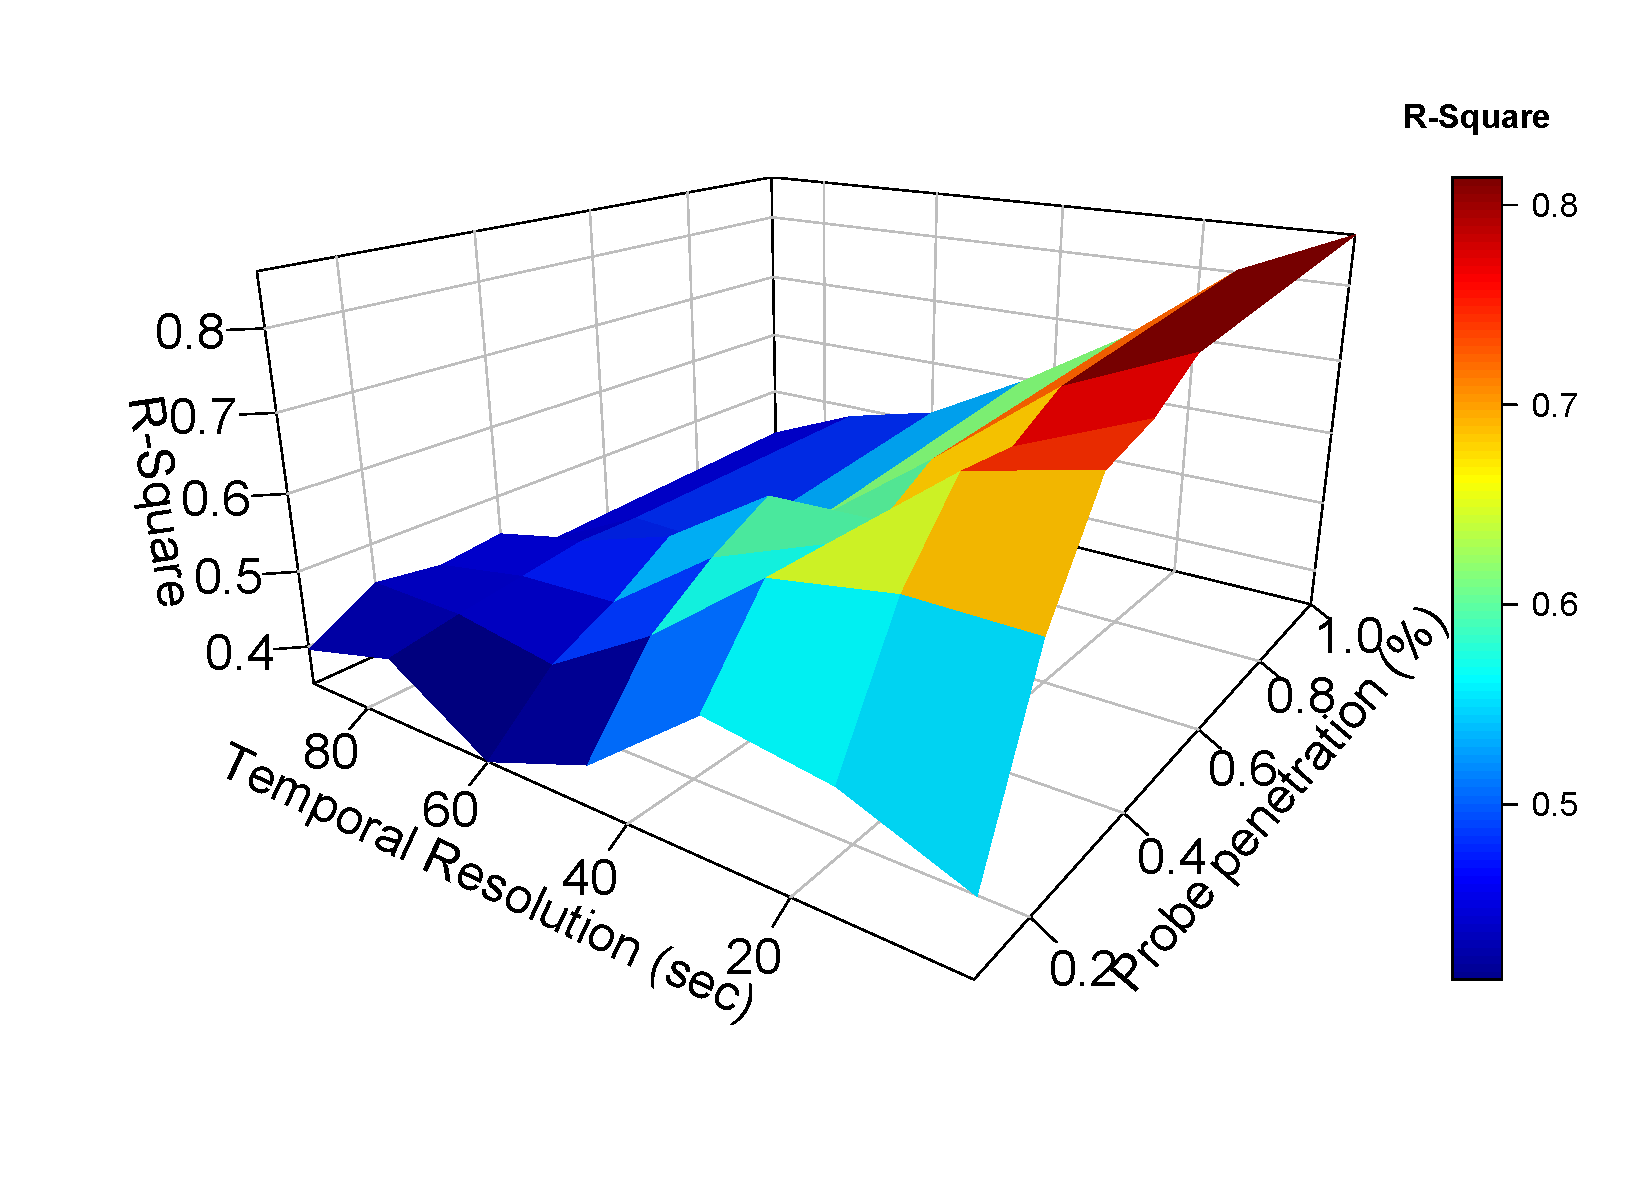
\includegraphics[clip=true,trim=1.0cm 2.8cm 0.5cm 1.7cm,scale=0.27]{graphs/Simulated/RSquare-sampling-freq-vs-penetration}
         	\caption{Temporal aggregation intervals}
         	 \label{fig:temporal-aggrgeation}
    \end{subfigure} 
   \caption{ Traffic flow and temporal resolution estimation for recursive binary splitting}
   \end{figure*}

Using the relation $Q=\rho\times \bar{V}$ the flow-density fundamental diagram is obtained as shown in Figure~\ref{fig:flow-density} at probe penetration of $10\%$. The average speed $\bar{V}$ and the density $\rho$ were aggregated using the recursive binary split for a two minute subinterval. The critical density for congestion ($\rho_{c}$) is around $100$ vehicles/km for P.I.E.

Figure~\ref{fig:temporal-aggrgeation} provides the average $R^2$ Statistic as a function of probe penetration and temporal aggregation intervals. Five two minute sub intervals of the  scenario shown in Figure~\ref{fig:heavy-traffic} were used for computing the aggregate $R^2$ Statistic. Clearly the accuracy of the density prediction decreases as the temporal aggregation interval increases. The graph indicates that acceptable accuracy of density estimates from FCD (when used in conjunction with binary splitting) is obtained at resolutions of around $15$ to $20$ seconds. This result thereby estimates the sampling period of probe vehicles required for traffic sate estimation. Increase of the probe sampling period to around $15$ seconds significantly reduces the computational resources required for real-time map matching and traffic state reconstruction. 



\section{Conclusions and Future Work}
\label{sect:future-work}

In this work we have established that reliably estimating traffic state and  more specifically density (and thereby flow) on an expressway can be achieved with a minimum of $5\%$ to $10\%$ probe vehicles depending upon the prevailing traffic conditions. Microscopic traffic simulations reveal that recursive binary partitioning can be used to subdivide a stretch of road to identify homogeneous regions of $Q, \rho$ and $\bar{V}$.

In the future, we would like to investigate if the results obtained on a relatively homogeneous expressway can be replicated on signalized urban street networks. Future work would also involve optimizing the minimum variance partitioning of the road network to automatically detect onset of congestion and anomalous events such as accidents based on statistical learning methods. Accurate estimation of speed, density and flows along important roads can help initialize data driven simulations for short term predictions of the evolution of traffic flows. Predictive simulations will play a major role in enhancing the capabilities of dynamic control strategies such as ramp metering and routing for traffic flow optimization.


\subsection{Acknowledgments}
\label{sect:acks}
This work was financially supported by the Singapore National Research Foundation under its Campus for Research Excellence And Technological Enterprise (CREATE) programme.

\label{sect:bib}
\bibliographystyle{plain}
\bibliography{demobib}


\end{document}
